\documentclass[UTF8]{article}

%设置页边距
\usepackage{geometry}
\geometry{left=2cm,right=2cm,top=2cm,bottom=2cm}
\usepackage{algorithm}  
\usepackage{algpseudocode}  
\usepackage{amsmath}  

%插入代码
\usepackage{titlesec}
\usepackage{listings}
\usepackage{xcolor}
\lstset{
    numbers=left,
    numberstyle=\scriptsize,
    keywordstyle=\color{red!80},
    commentstyle=\color{red!50!green!50!blue!50}\bf,
    frame=trbl,
    rulesepcolor=\color{red!20!green!20!blue!20},
    backgroundcolor=\color[RGB]{245,245,244},
    escapeinside=``,
    showstringspaces=false,
    xleftmargin=5em,xrightmargin=5em,
    aboveskip=1em,
    framexleftmargin=2em,
}

%设置中文
\usepackage{ctex}
\usepackage{tikz}
\usepackage{fancybox}
\usepackage{authblk}
\begin{document}

\title{网数大作业:新闻推荐系统报告}
\author[*]{熊兴旺}
\author[*]{温旭}
\author[*]{郑昕}
\author[*]{张嘉宝}
\affil[*]{计算技术研究所 \authorcr \{xiongxingwang,wenxu,zhengxin,zhangjiabao\}@ict.ac.cn}

\date{\normalsize\today}
\clearpage
\maketitle

\tableofcontents

\newpage
\section{简介}
	新闻推荐是指根据用户的点击记录,向用户推荐他们可能感兴趣的新闻。新闻推荐具有以下特点:
    \begin{enumerate}
        \item 最近几天的新闻更可能被浏览,很少会有人去浏览很久以前的新闻,所以尽量推荐较近的新闻;
        \item 热点新闻更容易引人注意;
        \item 相似的用户可能喜欢相似的新闻。
    \end{enumerate}
\section{相关工作}
\subsection{基于内容的推荐算法}
	将与用户点击过的新闻相似性较高的其他新闻推荐给用户。对新闻和用户进行分析以建立属性特征,利用此特征为用户推荐最为相似的新闻,关键在于如何计算新闻和用户的相似度。
	\begin{enumerate}
		\item 新闻特征提取:为每个新闻提取特征属性,比如表示为词向量。
        \item 用户特征提取:利用用户的浏览记录为每个用户提取特征属性,比如利用用户浏览过的新闻词向量构造用户向量。
        \item 为用户推荐与其相似度较高的新闻。
	\end{enumerate}

\subsection{协同过滤推荐算法}
不需要额外获取分析用户或新闻的内容属特性,是基于用户历史行为数据进行推荐的算法。
\subsubsection{基于用户的协同过滤算法}
将与当前用户有相同偏好的其他用户所喜欢的新闻推荐给当前用户。
	\begin{enumerate}
        \item 找到与目标用户喜好相似的邻居用户集合。
        \item 在邻居用户集合中,为用户推荐其感兴趣的新闻。
    \end{enumerate}
\subsubsection{基于物品的协同过滤算法}
为用户推荐那些与他们之前喜欢的新闻相似的新闻。
	\begin{enumerate}
        \item 根据用户历史行为数据,计算新闻间的相似度。
        \item 利用用户行为和新闻间的相似度为用户生成推荐列表。
    \end{enumerate}
\subsubsection{基于模型的协同过滤算法}
User-Based 或 Item-Based 方法共有的缺点是资料稀疏,难以处理大数据量下的即时结果,
因此发展出以模型为基础的协同过滤技术:先用历史数据训练得到一个模型,再用此模型进行预测。
\subsection{混合模型推荐算法}
	\begin{enumerate}
        \item 多个推荐算法独立运行,获取的多个推荐结果以一定的策略进行混合。
        \item 将前一个推荐方法产出的中间结果或者最终结果输出给后一个推荐方法。
        \item 使用多种推荐算法,将每种推荐算法计算过程中产生的相似度值通过权重相加,调整每个推荐算法相似度值的权重,以该混合相似度值为基础,选择出邻域集合,并结合邻域集合中的评估信息,得出最优的推荐结果。
    \end{enumerate}

\section{方法}
\subsection{KNN}
把样本中的所有新闻样本向量化。然后对于测试集中的所有用户,根据其已点击的新闻,计算平均新闻向量,然后通过最近邻算法查找最近$k$个向量推荐给用户。

对于新用户,系统推荐的是当前最热门的$k$条新闻。由于用户浏览的新闻往往都是最近的新闻,很少会有人去浏览很久以前的新闻,所以尽量推荐较近的新闻。在KNN实验中,只给用户推荐2014年1月1日后发表的新闻。

\subsection{SVD}
对于训练数据,构造用户-新闻矩阵$A$,将$A$分解为$USV^{T}$,其中$U$表示用户的主题分布,$S$表示奇异值,$V$表示新闻的主题分布。利用基于模型的协同过滤方法估计测试集:利用$USV^{T}$重建矩阵,并过滤掉已经评分的物品,对于每一行(一个用户)推荐值最大的几个新闻,对于从未在训练集中出现过的新用户推荐最近最热的新闻。
\subsection{NMF}
对于训练数据,构造用户-新闻矩阵V,将V分解为$W\times H$,其中W表示用户的主题分布,$H$表示物品的主题分布。利用基于模型的协同过滤方法估计测试集,利用$W\times H$重建矩阵,并过滤掉已经评分的物品,对于每一行(一个用户)推荐值最大的几个新闻,对于从未在训练集中出现过的新用户推荐最近最热的新闻。

\subsection{评价方法}
为了评价不同的推荐算法的推荐效果,我们让系统分别给测试集中的用户推荐10、40、100条新闻,然后将推荐新闻的命中数作为推荐算法的评价指标。

\section{实验}
\subsection{数据预处理}
数据集共31天,将前20天作为训练集,后11天作为测试集。

\paragraph{数据清洗} 删掉数据集中,新闻为NULL或404的新闻。由于新闻正文中的英文都没有断词,故把新闻中正文中的英文删除。
\paragraph{分词} 采用\textbf{jieba} 工具讲新闻标题、新闻正文进行分词。
\paragraph{特征分析} 

\subsection{KNN}
采用\textbf{CountVectorizer}文本向量方法提取新闻的特征向量。

\paragraph{KNN 效果} 给测试集中的每个用户请求,分别推荐10、40,100条新闻,总命中数分别为570、1377、2891,其中测试集中总共包含16646条记录。

图\ref{knn-example}展示了KNN 的推荐效果:
\begin{figure}[ht]
    \centering
    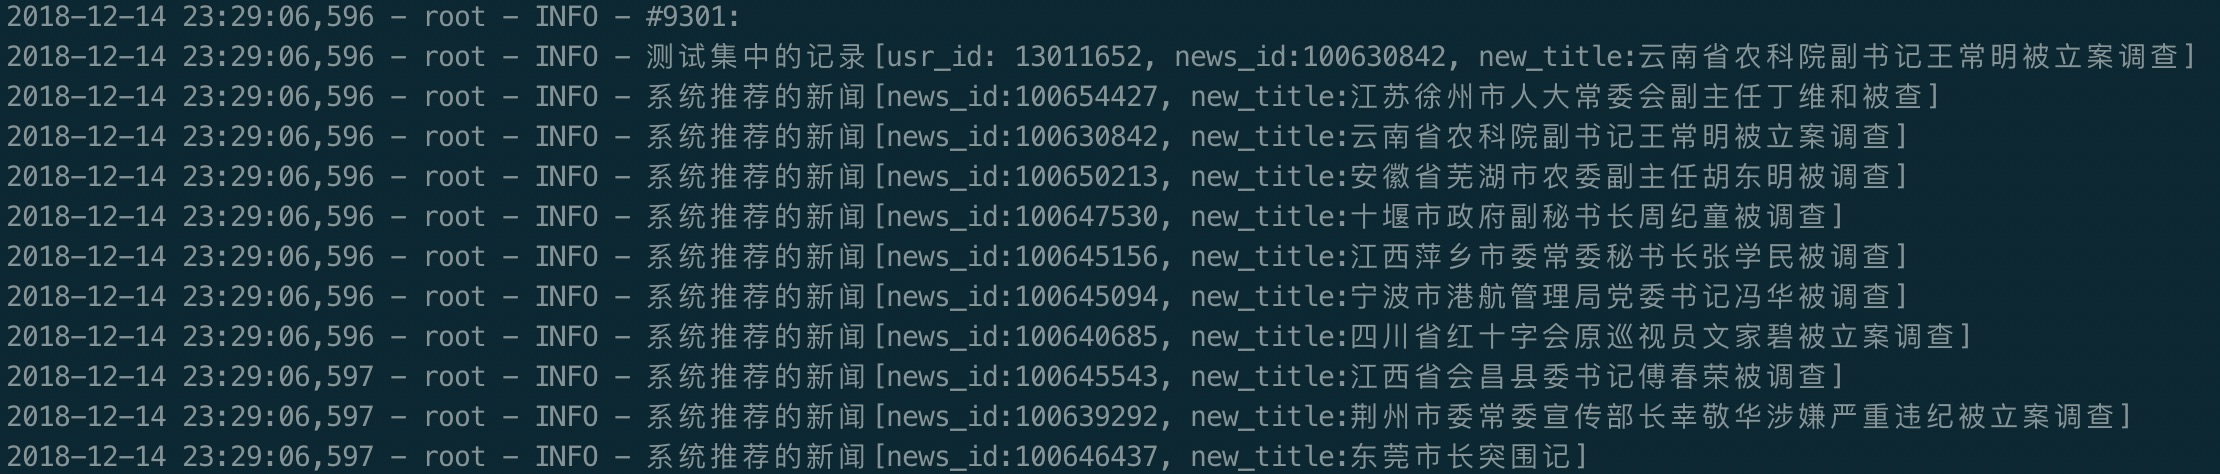
\includegraphics[scale=0.23]{./figures/knn-example.jpg}
    \caption{KNN 推荐效果}
    \label{knn-example}
\end{figure}

\subsection{SVD}
SVD效果:如果将后11天整体作为测试集,训练时间为19s,对于每个用户推荐10条新闻时总命中数为205;如果对于后11天每天进行推荐,比如利用前22天的数据预测第23天的数据,对于每个用户每天推荐10条新闻时总命中数为321。
%[8, 8, 10, 10, 9, 11, 10, 10, 11, 11, 10]s

SVD优点:考虑用户与用户,文档与文档之间的相似关系,训练集无需对文本进行处理,比较快。

SVD缺点:冷启动,测试集中有过半的新闻未曾在训练集中出现过,SVD无法对用户推荐这些新闻。

可能改进:利用混合模型,综合考虑内容过滤和协同过滤。
\subsection{NMF}
NMF效果:如果将后11天整体作为测试集,训练时间为30s,对于每个用户推荐10条新闻时总命中数为270;如果对于后11天每天进行推荐,比如利用前22天的数据预测第23天的数据,对于每个用户每天推荐10条新闻时总命中数为317。
%[21, 25, 50, 56, 61, 65, 60, 60, 61, 65, 66]

NMF优缺点与SVD相似。

尝试改进:尝试结合NMF与TF-IDF来处理新的新闻,未取得理想效果。


\section{方法2}
\subsection{算法简述}
使用nmf算法计算评分矩阵,基于item的协同过滤方法推荐训练集时间段内的老新闻;使用tfidf基于新闻标题计算相似度,推荐测试集时间段内的新新闻;统计点击率最高的老新闻和相似度与其最高的新新闻向新用户进行非个性化推荐。
\subsection{算法详述}
\subsubsection{关键词定义}
\begin{enumerate}
	\item 根据新闻的发布时间,将一个内所有新闻分为旧新闻和新新闻,旧新闻为前20天发布的新闻,新新闻为后10天发布的新闻。
	\item 根据用户是否在训练集中有点击记录将用户分为老用户(有点击记录)和新用户(没有点击记录)。
\end{enumerate}
\subsubsection{训练集划分}
根据用户对新闻单击动作的执行时间,即数据表中“访问页面时间“,将数据分成训练集和测试集,训练集为访问页面时间在前20天的记录,测试集为访问页面时间在后10天的记录。
\subsection{推荐策略}
系统对测试集中所有用户每人推荐10条新闻。根据用户性质的不同,推荐策略不同:
\subsubsection{向老用户的推荐方法}
\begin{enumerate}
	\item 使用nmf算法基于item的协同过滤向用户推荐k\_old条未看过的旧新闻。
	\item 使用tfidf算法基于新闻标题和正文计算新闻之间的相似度,向用户推荐(10 - k\_old)条新闻,由nmf算法得到的k\_hot条用户最喜欢的已读新闻推荐生成。
\end{enumerate}
\subsubsection{向新用户的推荐方法}
\begin{enumerate}
	\item 向用户推荐k\_old\_new条点击数最高的旧新闻。
	\item 使用tfidf算法基于新闻标题和正文计算新闻之间的相似度,向用户推荐(10 - k\_old\_new)条新新闻,由k\_hot\_new条点击数最高的旧新推荐生成。
\end{enumerate}
k\_old、k\_hot、k\_old\_new、k\_hot\_new皆为输入系统的参数。
\subsection{评价指标}
hit:推荐新闻与用户真实阅读的新闻之间交集的个数。
\subsection{设计理由}
本算法的推荐策略主要从2各方面考虑:用户自身兴趣和整体新闻热点。
\subsubsection{用户自身兴趣}
分析用户自身兴趣属于个性化推荐,能分析有浏览记录的用户,可通过分析用户点击历史来推测用户兴趣,故本算法选择使用nmf来计算用户在所有老新闻中的兴趣,推荐未读新闻中得分最高的老新闻,再使用基于内容的算法tfidf分析所有新新闻的标题,获得与这些老新闻主题最相近的新新闻。
\subsubsection{热点新闻}
对于训练集中没有浏览记录的用户视作新用户,由于没有用户的其他个人信息,故我们假设任何一位新用户都对当前对热点新闻感兴趣,故本算法先统计出老新闻中点击率最高者向用户推荐,同时使用tfidf基于新闻标题分析获得与这些老新闻话题最相似的新新闻向用户推荐。
\section{实验及分析2}
\subsection{实验结果}
系统向所有测试集用户(老用户2204人,新用户675人,共2879人),每人推荐10条新闻,累计共推荐28790次,实验结果如下:
基于新闻标题计算相似度的推荐结果:90。
基于新闻正文计算相似度的推荐结果:3。
\subsection{结果分析}
基于新闻标题的相似度计算和基于新闻正文结果相差较大,有可能是因为数据集中的新闻标题几乎都能够较好地概括新闻具体内容,而新闻正文中常带有背景介绍等内容,因此相似度计算结果没有分析标题的好。但基于标题的推荐hit值仍不够高,原因有肯能是因为标题太短。
\subsection{优点}
\begin{enumerate}
	\item 融合多种推荐方法,使用了协同过滤和基于内容的推荐方法,还考虑了非个性化推荐。
	\item 系统所使用的推荐逻辑:站在用户角度推荐最合适的新闻,比站在新闻角度分发给最适合的用户,更符合推荐系统的业务逻辑,因此实验结果hit更高。
\end{enumerate}
\subsection{缺点及解决方案}
\subsubsection{特征分析不完备}
算法未使用新闻发布时间、用户点击时间两种数据,可以通过分析两种数据之间的关系,进一步分析用户兴趣的相关因素,例如:用户是否偏好阅读发布时间与现在相近的新闻,用户点击时间与新闻发布时间之差是否能体现用户兴趣。
\subsubsection{协同过滤算法不够吻合}
使用的协同过滤算法nmf与题目的假设并不完全吻合:nmf主要用于用户对物品的评分矩阵分析,而本题数据为用户点击记录,即用户与新闻同时出现的概率,应使用基于概率假设的算法,例如plsi。本次实验由于时间因素未能在截止前实现,后续考虑尝试。
\subsubsection{基于新闻标题的推荐方法中标题太短}
由于新闻第一段通常是对全文对综述,而第一段比标题长,又比正文短,故可以尝试使用基于新闻正文第一段来计算新闻相似度。

\end{document}
